%%%%%%%%%%%%%%%%%%%%%%%%%%%%%%%%%%%%%%%%%%%%%%%%%%%%%%%%%%%%%%%%%%%%%%%%%%%%%%%%
%2345678901234567890123456789012345678901234567890123456789012345678901234567890
%        1         2         3         4         5         6         7         8

\documentclass[letterpaper, 10 pt, conference]{ieeeconf}  % Comment this line out if you need a4paper

%\documentclass[a4paper, 10pt, conference]{ieeeconf}      % Use this line for a4 paper

\IEEEoverridecommandlockouts                              % This command is only needed if 
                                                          % you want to use the \thanks command

\overrideIEEEmargins                                      % Needed to meet printer requirements.

%In case you encounter the following error:
%Error 1010 The PDF file may be corrupt (unable to open PDF file) OR
%Error 1000 An error occurred while parsing a contents stream. Unable to analyze the PDF file.
%This is a known problem with pdfLaTeX conversion filter. The file cannot be opened with acrobat reader
%Please use one of the alternatives below to circumvent this error by uncommenting one or the other
%\pdfobjcompresslevel=0
%\pdfminorversion=4

% See the \addtolength command later in the file to balance the column lengths
% on the last page of the document
\usepackage{graphicx}
\usepackage{setspace}
\usepackage{subfigure}
\usepackage{mathptmx}
\usepackage{bm}
\usepackage{amsmath,amssymb} % define this before the 
\usepackage{color}
\usepackage{algorithm}
\usepackage{algpseudocode}
\usepackage{enumerate}
\usepackage{epstopdf}
\usepackage{array}  
\usepackage{eqparbox}
\usepackage{multirow}
\epstopdfsetup{update}
\usepackage{url}
\usepackage{mathtools}
\usepackage{hyperref}
\usepackage{adjustbox}
\usepackage{caption}
\pdfminorversion=4


\graphicspath{ {./figures} }
\title{\LARGE \bf
Deep Flow Guided Image Based Visual Servoing 
}


\author{Y V S Harish$^{1}$,  Harit Pandya$^{2}$, Ayush Gaud$^{3}$, Shreya Terupally$^{1}$ and K. Madhava Krishna$^{1}$ % <-this % stops a space
%\thanks{*This work was not supported by any organization}% <-this % stops a space
\thanks{$^{1}$IIIT Hyderabad, India,
        {\tt\small harish.y@research.iiit.ac.in, \hspace{5mm} mkrishna@iiit.ac.in}}%
\thanks{$^{2}$University of Lincoln, UK,
        {\tt\small hpandya@lincoln.ac.uk}}%
\thanks{$^{3}$Mathworks, India,
        {\tt\small ayush.gaud@gmail.com}}%
}




\begin{document}


\newpage
\maketitle
\thispagestyle{empty}
\pagestyle{empty}


%%%%%%%%%%%%%%%%%%%%%%%%%%%%%%%%%%%%%%%%%%%%%%%%%%%%%%%%%%%%%%%%%%%%%%%%%%%%%%%%
\begin{abstract}

Existing deep learning based visual servoing approaches regress the relative camera pose between a pair of images circumventing the requirement for scene's depth and camera parameters. However, estimation of accurate camera pose on diverse scenes is a non-trivial problem, thus existing deep learning based approaches require a huge amount of training data and sometimes fine-tuning for adaptation to a novel scene.
Furthermore, current approaches do not consider underlying geometry of the scene and rely on direct estimation of camera pose. Thus, inaccuracies in prediction of the camera pose especially for distant goals leads to a degradation in the servoing performance. In this paper, we propose a two-fold solution: (i) We consider optical flow as our visual features, which are predicted using a deep neural network. The flow features provide dense correspondences between an image pair that leads to a precise convergence of the servoing approach. (ii)  We then integrate these flow features with depth estimate provided by another neural network using interaction matrix similar to classical image based visual servoing. This geometrical understanding provided by the depth integration increases the robustness of the overall system. We present two paradigms for depth estimation under single-view and two-view settings. Through 10 unseen photo-realistic simulation environments and a real scenario on an aerial robot, we show that our approach generalises to novel scenarios producing precise and robust servoing performance for 6 degrees of freedom positioning task over diverse environments with even large camera transformations without any requirement for retraining or fine-tuning. 

%
\end{abstract}

%The control problem is then solved my iterative minimizing the error between the visual features extracted from the current and the desired pose \cite{vsbasic}.
%%%%%%%%%%%%%%%%%%%%%%%%%%%%%%%%%%%%%%%%%%%%%%%%%%%%%%%%%%%%%%%%%%%%%%%%%%%%%%%%
\section{INTRODUCTION}
Visual servoing addresses the problem of attaining a desired pose with respect to a given environment using image measurements from a vision sensor. Classical visual servoing approaches extract a set of hand-crafted features from the images. Pose based visual servoing (PBVS) approaches use these visual features to estimate the camera pose directly in Cartesian space from a given image. The controller then guides the robotic system in the direction that minimizes the difference in pose between current and desired image pair directly in 3D space. Whereas, image based visual servoing (IBVS) approaches control the robot by minimizing the feature error explicitly in the image space \cite{vsbasic}. It can be observed that the pose based visual servoing controllers attain the desired pose without getting stuck at local minimas. They, however, are sensitive to camera calibration errors and pose estimation errors \cite{vsprob}. On the contrary, image based visual servoing approaches are robust to calibration and depth errors but could lead to a local minima. Classical PBVS and IBVS approaches, both rely on reliable matching of hand-crafted features, thus inaccuracies while obtaining correspondences degrades the servoing performance. Direct visual servoing \cite{photometricvs} approaches avoid the feature extraction step and operates directly on image measurements. This helps in achieving higher precision in goal reaching, but the trade-off is a smaller convergence basin. Another rigid requirement of classical visual servoing approaches is the knowledge of environment's depth. This is especially difficult to obtain on robotic systems using a monocular camera.

\indent To circumvent the requirement for extracting and tracking hand-crafted features, 
Saxena et al. \cite{servonet} presented a deep learning based visual servoing approach. Specifically, they employed a deep network to estimate the relative camera pose, from an image pair. A traditional PBVS controller is then used to minimize the relative pose between the current and the desire image. Their network was trained on publicly available Microsoft 7 scenes dataset \cite{7scene} for estimating relative camera pose. Although trained on limited number of scenes, their network was able to generalise well on novel environments, however, the convergence basin was limited. Bateux et al. \cite{trainingdeepvs} presented a similar deep pose based visual servoing approach with a Siamese \cite{siamese} based network architecture for estimating relative camera pose from an image pair. They further proposed  extensive guidelines for training deep networks for the task of visual servoing. They used LabelMe database \cite{labelme} which contains a diverse set of images with scene variations while using homography for obtaining viewpoint variations to make the network robust. The network was then trained to estimate the relative pose given a pair of images taken from these viewpoints, which helped in generalisation of the approach in to different environments.  Similarly, Yu et al. also present a Siamese style deep network for visual servoing \cite{siamesevs}, their network obtains a much higher sub-millimeter precision for the servoing task, however the network was trained only on a table-top scene with similar objects and therefore requires retraining for adjusting to novel environments. 

%these approaches are closer to PBVS, where given a pair of images, the network estimates the relative pose between them and use a  
%recent visual servoing approaches employ deep neural networks.  
%presented a network Flownet \cite{flownet}  and 

\begin{figure*}[ht!]
    \begin{center}
    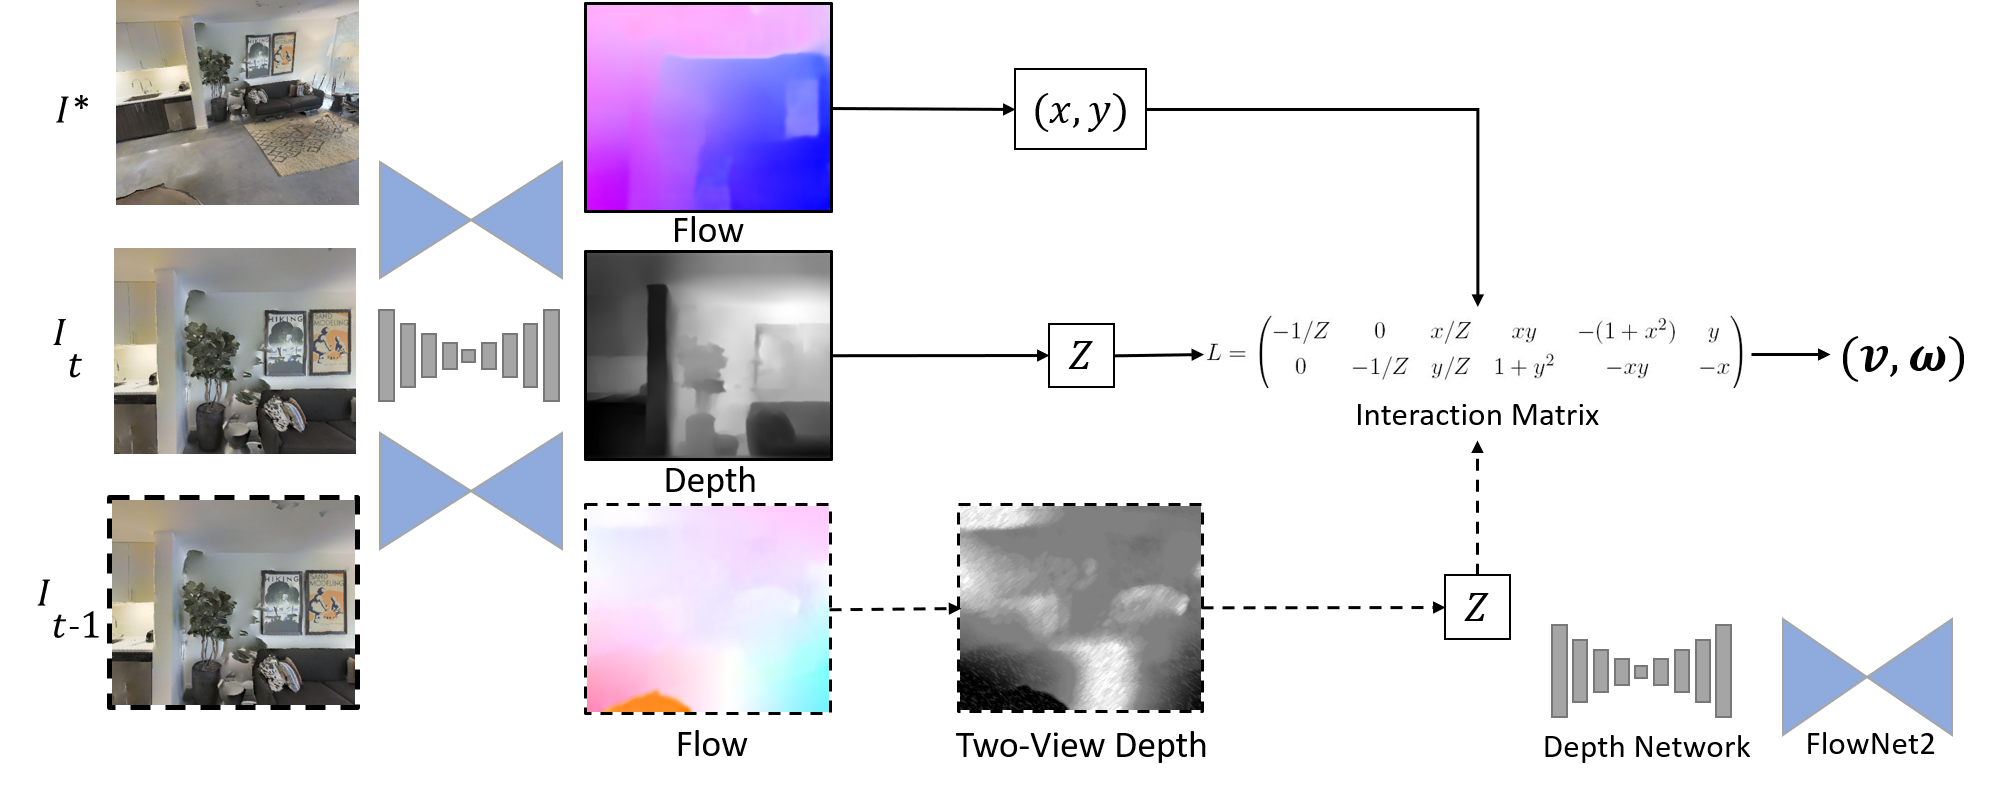
\includegraphics[width=17cm, height=7.0cm] {figures/Pipeline_VS.png}
    \caption{Pipeline of the proposed approach. We employ Flownet-2 network to estimate the feature error between current and desired pose. To predict the scene's depth at the current pose, we propose two designs: (i) We employ a depth-network to estimate depth from a single view. (ii) Alternatively, a scaled version of flow could also be used as disparity to achieve scene agnostic depth prediction. Finally, we combine the cues from depth and visual features using an interaction matrix similar to classical IBVS. This helps us in achieving a robust and precise visual servoing.}
    \label{fig:pipeline}
    \end{center}
\end{figure*}


\indent Unlike the above approaches that estimate the relative camera pose and use a PBVS controller for achieving the desired pose, recent deep reinforcement learning based visual servoing approaches \cite{sim2real,sim2real2}, \cite{deepq,sefsupervised} use neural controllers to maximize the rewards and therefore require minimal supervision. However, several of these approaches are specific to manipulation tasks and are trained only for scene with objects lying on a table. Furthermore, these approaches do not consider full 6 degrees of freedom (DOF) visual servoing. Sampedro et al.  \cite{deeprlvsdrone} showcased a similar deep reinforcement learning approach for an aerial robot for autonomous landing on a moving target, however they only report results for a single scene with a colored target. Zhu et al. \cite{targetdriven} presents the results quite similar to ours on a wide range of environments. Although, they constrain the motion to a plane and their approach is showcased on similar environments, thus generalisation on novel environments is non-trivial and requires fine tuning. %\cite{http://www.roboticsproceedings.org/rss15/p55.pdf}



\indent In this paper, we present a visual servoing approach based on deep learning for attaining a 6 DOF pose, which effectively generalises to novel environments. In contrast to existing approaches that directly attempt to estimate the relative pose between current and desired pose, we compute the dense correspondences using an optical flow network. These are combined with depth estimates from another network in a principled manner using interaction matrix. Integration with the scene
allows the network in achieving a large convergence basin and more generalisation to novel environments. To benchmark against existing deep visual servoing approaches, we extensively evaluate them on numerous perception and control criteria in photo-realistic simulation environments. Our approach not only attains precise convergence but it  also showcases larger convergence basin as compared to existing approaches. \\                   


Our contributions are summarized as follows:
\begin{itemize}

    \item We propose a novel system consisting of deep neural networks that systematically integrates depth cues with flow features. Our approach exhibits precise positioning even for distant goals, where existing approaches fails to converge. Our model also is able to generalise in diverse environments both indoors and outdoors effortlessly without any need for fine-tuning or retraining unlike other approaches \cite{targetdriven}.
    
    \item We present an extensive benchmark for deep servoing methods evaluating both perception and control performance on a variety of parameters such as, photometric error, camera poses error, trajectory length, smoothness of control commands and convergence basin. We showcase state-of-the-art performance under this comprehensive evaluation in table \ref{tbl:bench_quant}.
    
    \item We make our implementation and the pipeline to benchmark visual servoing approaches publicly available. It consists of photo-realistic scenes classified into three categories as easy, medium and hard based on the scene texture and convergence basin. It will help in facilitating fair and quantitatively thorough comparison of various visual servoing schemes. 

\end{itemize}


\section{Approach}
Existing deep visual servoing approaches aim to directly estimate the relative camera pose between the current and the desired pose in a PBVS style, therefore these approaches require a data sample for every iteration. This amounts to a huge amount of training data which is difficult to obtain. So, Bateux et al. \cite{trainingdeepvs} trained their network using dataset generated on a planar scene from multiple viewpoints in a simulation environment. Moreover, by selecting the textures from a variety of backgrounds, generalization could be achieved over different environments. Although, due to the incorrect depth of the scene, it is non-trivial to attain large camera transformations. Saxena et al. \cite{servonet} on the other hand, train their data by sampling image pairs from a given trajectory, as a result they trained their network on a limited dataset acquired from just seven environments. Yu et al. \cite{siamesevs} trained their networks only on a single table-top setting.

\indent To circumvent these strict training requirements, we base our approach on image based visual servoing. We employ a flow network \cite{flownet2} to estimate dense correspondences between current view and desired view. These visual features are easier to observe as compared to the relative pose estimates. Furthermore, to capture the geometry of the scene, we pivot our approach on depth cues similar to classical image based visual servoing. However, unlike classical IBVS, where a coarse depth was assumed, we are able to estimate the depth by using a deep network. In this work, we present two designs for obtaining the depth, in the first method we explicitly use a depth network \cite{depthnet} while our second design employs a scaled version of flow as a proxy for the depth. Our pipeline is illustrated in figure \ref{fig:pipeline}.

\subsection{Flow as visual features}
Classical IBVS approaches use local appearance based features such as SURF \cite{surf}, SIFT \cite{sift} to describe the scene and the feature error is computed by the difference between their locations in the current and the desired image ($s-s^*$). This requires accurate tracking of the visual features. However, for low textured environments, the number of feature detections are less, this combined with large matching inaccuracies results in incorrect error estimates. Whereas, optical flow provides dense correspondences even in case of low textured environments. Therefore, in this work we use optical flow to estimate the feature error between the current and the desired image ($\mathcal{F}(I_t,I^*)$). For estimating the visual feature error, we use the FlowNet-2 \cite{flownet2}, which is state-of-the-art in flow computation.

\subsection{Depth estimation}
Recent deep visual servoing approaches directly estimate the camera pose without accounting for the geometry of the underlying scene. This increases the estimation errors for distant goal which in turn reduces the convergence basin. For instance, Bateux et al. \cite{trainingdeepvs} trained their network on planar scenes and report sharp decrease in converge ratio for distance greater 2.5 cm and angle greater than 15 degrees. Similarly, Saxena et al. \cite{photometricvs} estimate the relative translation and rotation individually and thus require a scaling factor to fuse them.

\indent Even for the classical image based visual servoing approaches, depth plays a crucial role in their convergence in 3D environments. In the absence of knowledge of true depth of the scene, classical IBVS approaches either approximate the true depth through a coarse depth \cite{vsbasic}, or estimate the depth online \cite{onlinedepth} by observing the robot's odometry. Which, again limits the convergence basin especially in scenarios involving large camera transforms. In this paper, we present two designs to accommodate depth cues for stable visual servoing described in the sections below.

\begin{figure}
\centering
\begin{tabular}{cccc}
  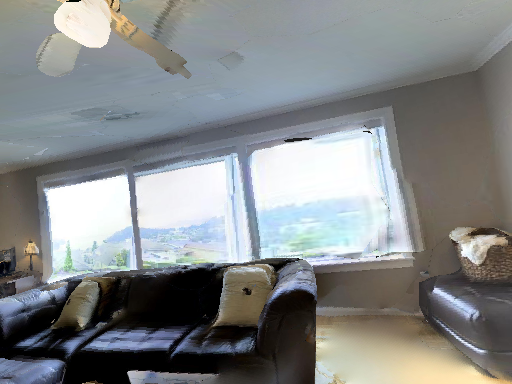
\includegraphics[width = 1.9cm, height=1.8cm]{comparison/scene_new.png} \hspace{-1em}  & 
  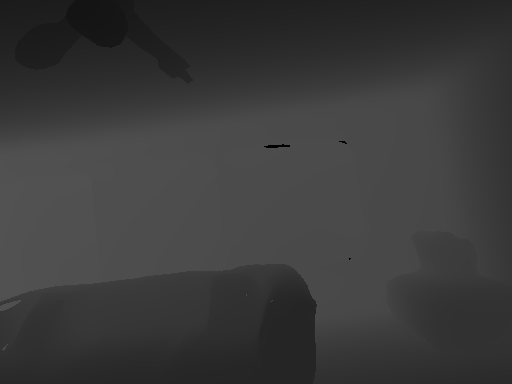
\includegraphics[width = 1.9cm, height=1.8cm]{comparison/depth_sensor_new.png} \hspace{-1em}  &
  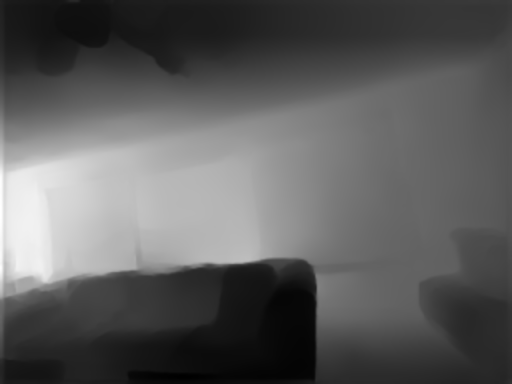
\includegraphics[width = 1.9cm, height=1.8cm]{comparison/depth_net_new.png}  \hspace{-1em} &
  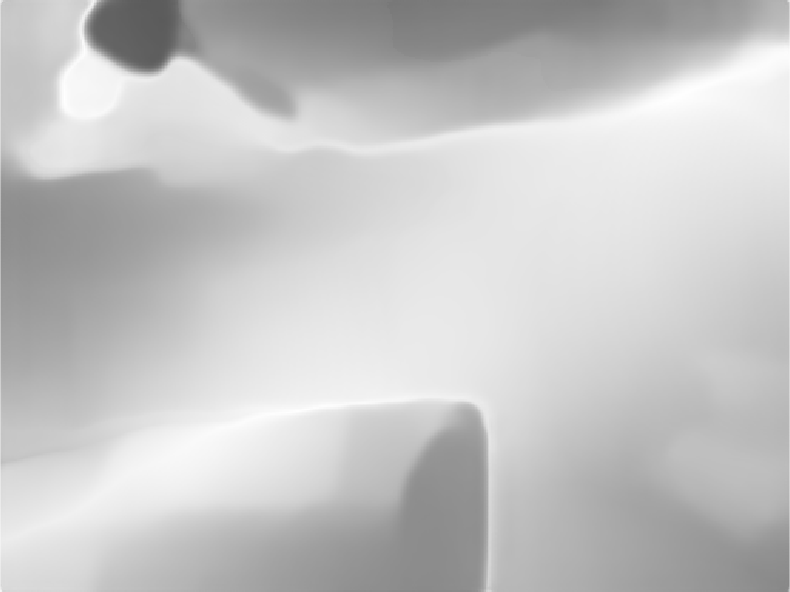
\includegraphics[width = 1.9cm, height=1.8cm]{comparison/flow_depth_new.png}  \hspace{-1em} \\
  (a) & (b) & (c) & (d)
\end{tabular}
\caption{(a) Given image, (b) True depth from the depth sensor, (c) single view from Depth Network and (d) two-view depth visualization from flow network between current and desired image.}
\label{fig:depth_comparision}%
\end{figure}

\subsubsection{Single view depth estimation}
Our first design is based on directly estimating scene's depth from single image. We employ an encoder-decoder based convolutional neural network architecture proposed by Alhashim et al. \cite{depthnet}. Authors inspire their encoder design from the DenseNet-169 \cite{densenet}, whereas the decoder is composed of 3 up-sampling blocks, each consisting of an up-sampling layer which is then concatenated with respective layer from encoder, similar to the U-net \cite{unet} and is followed by 2 convolution layers. They train their network on NYU-Depth-v2 dataset  \cite{nyudepthv2} on a 50K images and on  on a subset of around 26K images selected from KITTI dataset \cite{kitti}. %Having trained on both indoor and outdoor dataset, authors report that their network generalises on other indoor datasets as well.


\subsubsection{Two view depth estimation}
The  depth network proposed in the previous sub-section can estimate the scene's depth from a single image, however it requires extensive training on a large dataset. To achieve scene agnostic depth prediction, as an alternate, we propose to estimate depth using an image pair. Specifically, magnitude of optical flow could be seen as an inverted scaled representation of underlying depth. We again rely on our flow network to compute the optical flow between current and previous image and use it as a proxy for the depth, which allows the network to generalise across a diverse set of indoor and outdoor scenes. %as the depth is pivoting on a pair image and not just a single image. 

\indent Figure \ref{fig:depth_comparision} compares the depth of an indoor scene estimated from both the approaches  as compared to the ground truth depth of the scene given by the depth sensor of our simulation engine. It can be easily seen that depth network does a much better job in predicting the depth but it was trained on indoor objects, however the two-view depth captures the geometry of the scene at a coarser level without any fine-tuning or refinement.   

\subsection{Image based visual servoing}
Classical visual servoing approaches consider sparse correspondences between the current and desired configuration and minimize them iteratively using gradient descent over feature error in image space and pseudo-inverse of image Jacobian. On the other hand, we use a deep network \cite{flownet2} for estimating the dense correspondences as optical flow. Due to large dimensionality of the feature vector we employ levenberg-marquardt based gradient descent similar to  collewet et al. \cite{vssetfree}, specifically our control law describing the camera velocity $v_c$ is given as: 
\begin{equation}
v_c = - \lambda (L^TL+\mu diag(L^TL))^{-1} \mathcal{F}(I_t,I^*).    
\end{equation}
Where, the visual feature error is given by dense correspondences observed by the flow network. $L(z)$ is the interaction matrix as described in \cite{vsbasic} and the depth $z$ is estimated by either the depth network $D(I_t)$ or the scaled flow $\alpha  \mathcal{F}(I_t,I_{t-1})^{-1}$. The tunable parameters $\lambda$ and $\mu$ adjust the step size and direction of the descend respectively.

\section{EXPERIMENTS}
The motivation of the current work is to achieve an off-the-shelf scene agnostic visual servoing. Several deep visual servoing approaches \cite{sim2real,sim2real2,deepq,sefsupervised} only focus on goal reaching task for manipulation and do not consider the pose in which object is reached. A few approaches such as \cite{trainingdeepvs,siamesevs} do consider a 6 DOF goal reaching task, however their test-cases are limited to planar or near-planar scenarios like a table-top. Only \cite{photometricvs} provide results for 6 DOF goal reaching task for non-planar scenes, however they do not show results in a photo-realistic environments. The difference between the environments used for the servoing task could easily be noticed in figure \ref{fig:benchmark}.  The central focus in the experiments is to validate the ability to generalise on different environments. Therefore, we present a set of benchmarking tasks in simulation environment to be performed without fine-tuning the network. To showcase that our approach can be used as plug-and-play for various environments, we further present results with an aerial robot on an outdoor scenario. 

\begin{figure}
\begin{tabular}{c}    
  %\parbox[t]{0.1mm}{\rotatebox[origin=c]{90}{\hspace{4mm}Existing}} &
  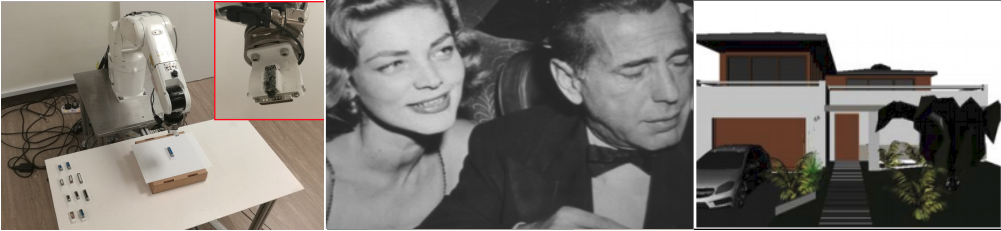
\includegraphics[width=7.9cm, height=2.1cm]{Dataset_images/bench_others_h.png} \\
  %\parbox[t]{0.1mm}{\rotatebox[origin=c]{90}{\hspace{4mm}Ours}} &
  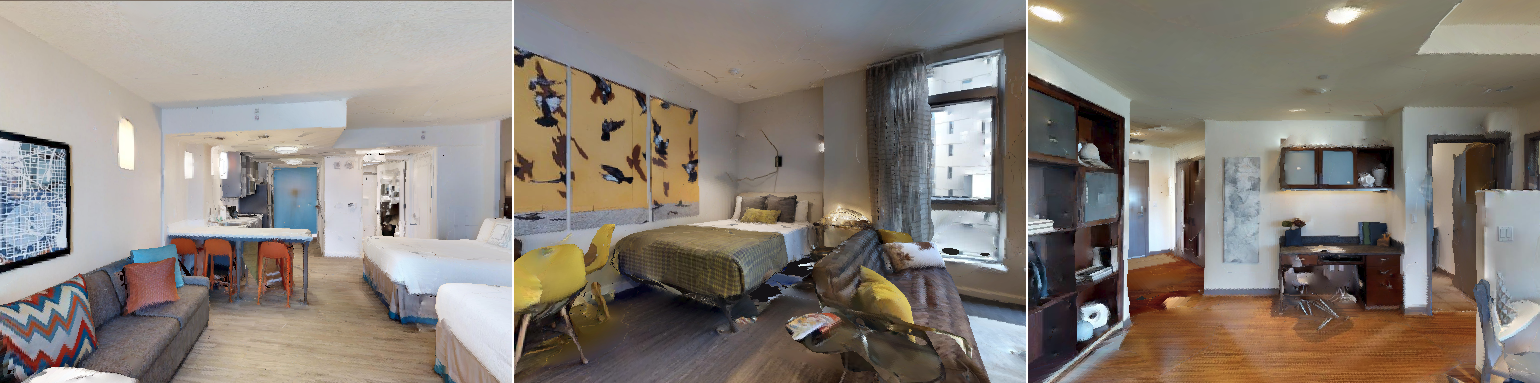
\includegraphics[width=7.9cm, height=2.1cm]{Dataset_images/bench_ours_h.png}
\end{tabular}
    \caption{The test-beds compared by existing deep visual servoing approaches (top) are either planar, near -planar(table-top) or synthetic. On the other hand, we propose a photo-realistic benchmark (bottom) for deep visual servoing approaches.}
    \label{fig:benchmark}
    
\end{figure}

\subsection{Simulation results on Benchmark}
The proposed simulation benchmark consists of 10 indoor photo-realistic environments from Habitat simulation engine \cite{habitat}. We have selected these scenes such that they cover different textures and variable number of objects. Further for each scene we provide an initial pose and a desired pose. We classify these tasks in three categories easy (refer figure \ref{fig:bench_qual}row 1-3), medium (refer figure \ref{fig:bench_qual}row 4-7)and hard (refer figure \ref{fig:bench_qual}row 8-10). The labeling is done based on amount of texture present in the scene and the difference between initial and desired pose. To evaluate the visual servoing approaches we propose following metrics capturing both perception as well as control aspects of servoing: final translation error, final rotation error, trajectory length, number of iterations and  time per iteration and smoothness of trajectory. We report both quantitative \ref{tbl:bench_quant}  and qualitative \ref{fig:bench_qual} results on the benchmark. It can be noticed that Saxena et al. \cite{servonet}, are able to converge on easy and medium scenes but they have difficulty on hard scenes. We also compared with photometric visual servoing, for the comparison we provided true depth of the scene obtained from the depth sensor. It can be seen from the  table \ref{tbl:bench_quant} even with the knowledge of the correct depth of the scene, it is not able to converge in most of the environments. Also the quantitative results (table \ref{tbl:bench_quant}) show that depth predicted by our approaches (single-view as well as view) are at par with the sensor depth for visual servoing tasks. We obtain a precise final positioning error of 2 cm over a 2 m trajectory and the rotation error is under 1 degree.

\begin{table}[h!]
\begin{center}
   \begin{tabular}{|c|c|c|c|c|c|c|}
\hline
Metric & I. err & \cite{photometricvs} & \cite{servonet} & T.depth & D.net & F.depth \\ \hline
\hline \hline
T. err &1.42 & 0.06 & 0.19 & 0.02 & 0.02 & 0.04 \\\hline
R. err & 18.20 & 0.76 & 0.89 & 0.37 & 0.38 & 0.72 \\  \hline
 Tj. len & - &2.26 & 2.69 &  2.24  &  1.42  &  1.19  \\ \hline
 Iter& - & 956 & 1486   &  764  &  233  &  1560  \\ \hline
\hline
T. err & 1.79 & 0.12 & 0.08 & 0.04 & 0.02 & 0.03 \\\hline
R. err & 16.33 & 0.66 & 0.84 & 0.84 & 0.42 & 0.06 \\  \hline
 Tj. len & - & 2.22 & 2.48  &  1.58  &  1.55  &  2.31  \\ \hline
 Iter& - & 869 &  1687  &  150  &  143  &  871  \\ \hline
\hline
T. err &1.41 & 0.28 & 0.13 & 0.04 & 0.02 & 0.04 \\\hline
R. err& 18.07 & 3.23 & 6.44 & 8.72 & 8.87 & 8.39 \\  \hline
 Tj. len &  - & NC & 2.94  &  2.31  &  1.19  &  1.1 \\ \hline
 Iter& - & NC & 1647  &  214  &  185  &  580  \\ \hline
\hline


\hline  \hline
T. err &1.15 & 0.91 & 0.83 & 0.02 & 0.02 & 0.02 \\ \hline
R. err& 17.27 & 13.25 & 10.54 & 1.39 & 1.38 & 0.66 \\  \hline
 Tj. len & - & NC & NC  &  1.52  &  2.56  &  0.89  \\ \hline
 Iter& - & NC & NC  &  104  &  186  &  3831  \\ \hline
 \hline
T. err &1.64 & 0.33 & 0.04 & 0.03 & 0.03 & 0.03 \\ \hline
R. err& 30.96 & 3.57 & 1.39 & 0.85 & 0.83 & 0.89 \\  \hline
 Tj. len & - & NC & 2.86  &  2.36  &  3.65  &  2.37 \\ \hline
 Iter&- & NC & 1235  &  84  &  89  &  869  \\ \hline
\hline
T. err &1.37 & 1.29 & 1.25 & 0.03 & 0.02 & 0.01 \\\hline
R. err& 17.26 & 7.63 & 9.55 & 1.81 & 0.77 & 1.81 \\  \hline
 Tj. len & - & NC & NC  &  1.33  &  2.49  &  1.26  \\ \hline
 Iter& - & NC & NC  &  20  &  283  &  661  \\ \hline
 \hline
T. err &1.95 & 0.54 & 0.35 & 0.02 & 0.02 & 0.03 \\ \hline
R. err& 22.86 & 4.56 & 6.47 & 0.53 & 0.53 & 1.39 \\  \hline
 Tj. len &- & NC & NC  &  2.74  &  2.82  &  1.85  \\ \hline
 Iter& - & NC & NC  &  62  &  244  &  981  \\ \hline
\hline

\hline \hline
T. err &2.54 & 2.49 & 2.32 & 0.03 & 0.01 & 0.02 \\\hline
R. err& 20.02 & 39.65 & 48.77 & 11.67 & 0.34 & 0.55 \\  \hline
 Tj. len & - & NC & NC  &  2.03  &  5.88  &  2.26  \\ \hline
 Iter& - & NC & NC  &  504  &  237  &  754  \\ \hline
\hline
T. err &1.94 & 2.36 & 2.27 & 0.04 & 0.041 & 0.041 \\ \hline
R. err& 31.78 & 43.37 & 29.69 & 0.78 & 0.75 & 0.91 \\  \hline
 Tj. len &  - & NC & NC  &  2.24  &  2.28  &  2.32  \\ \hline
 Iter& - & NC & NC  &  183  &  145  & 1124  \\ \hline
\hline
T. err &2.43 & 2.27 & 1.36 & 0.01 & 0.01 & 0.02 \\ \hline
R. err& 36.05 & 53.246 & 29.24 & 0.28 & 0.16 & 0.49 \\  \hline
 Tj. len & - & NC & NC  &  2.52  &  2.67  &  3.52  \\ \hline
 Iter& - & NC & NC  &  314  &  114  &  1386  \\ \hline

      \end{tabular}
\caption{Quantitative results on benchmark. We compare our all the 3 variants True depth (T. depth), Depth network (D.net) and Flow depth (F.depth), of our approach with existing visual servoing approaches and report following metrics Initial error (I. err) final translation error( T. err), rotation error( R. err), trajectory length (Tj. len). It can be observed that existing approaches are able to converge only on the simple scenes, whereas our approaches converge till }
 \label{tbl:bench_quant}
 \end{center}
 \end{table}
\begin{figure*}[h!]
\begin{center}

%\begin{adjustbox}{width=0.5\textwidth,height=57mm,center} 

\begin{tabular}{|c| c |c | c | c | c | c|}
\hline
 Initial Image &Desired Image&PhotoVS&Saxena et al.\cite{servonet}& True depth &  Depth-net & Flow-depth  \\ \hline
\hline \hline
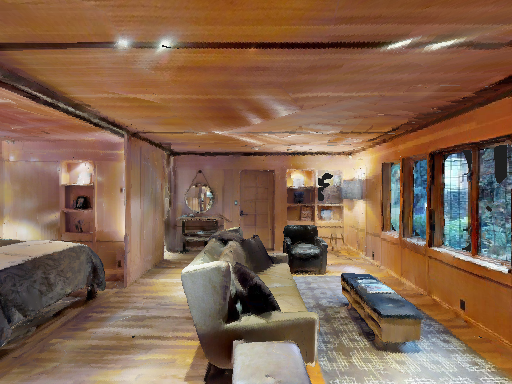
\includegraphics[width=18mm, height=17mm]{TrueDepth/ROANE/init.png} &   
            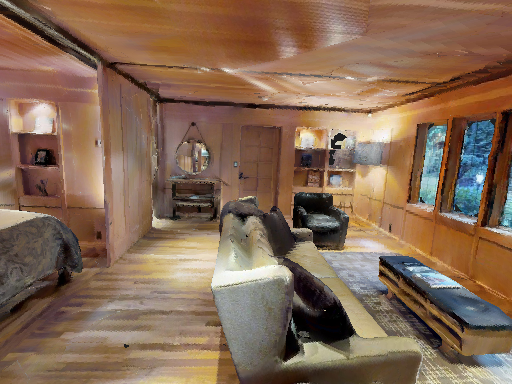
\includegraphics[width=18mm, height=17mm]{TrueDepth/ROANE/des.png} & 
            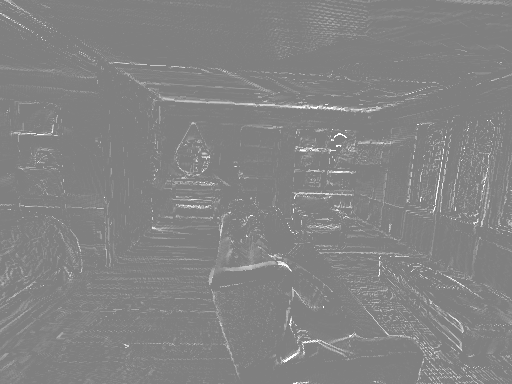
\includegraphics[width=18mm, height=17mm]{PhotoVS/ROANE/ferror.png} & 
          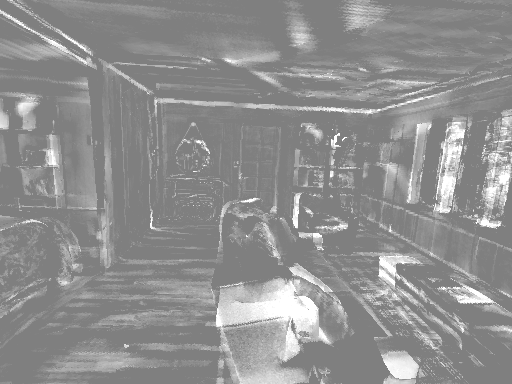
\includegraphics[width=18mm, height=17mm]{ICRA17/ROANE/ferror.png} & 
 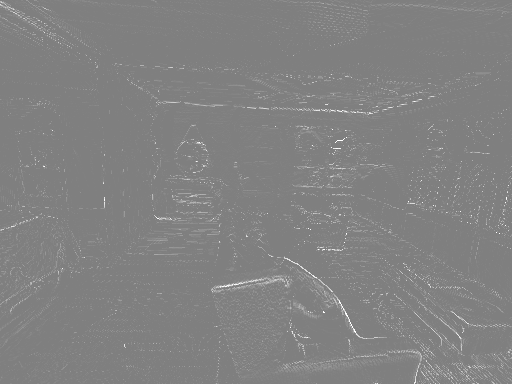
\includegraphics[width=18mm, height=17mm]{TrueDepth/ROANE/ferror.png} &
  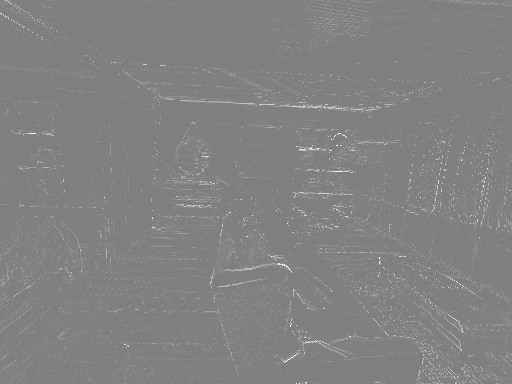
\includegraphics[width=18mm, height=17mm]{DepthNetwork/ROANE/ferror.png} &
  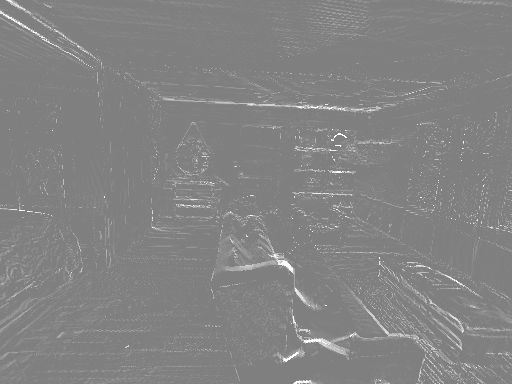
\includegraphics[width=18mm, height=17mm]{FlowDepth/ROANE/ferror.png}

 \\ \hline
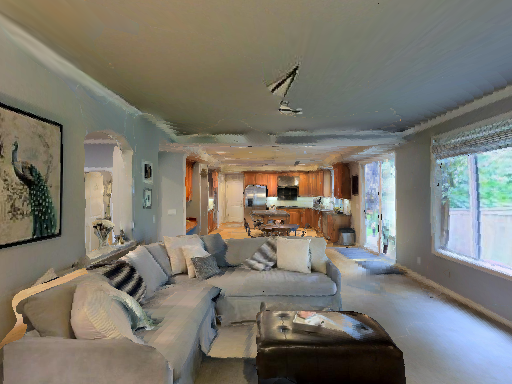
\includegraphics[width=18mm, height=17mm]{TrueDepth/BALLOU/init.png} &   
            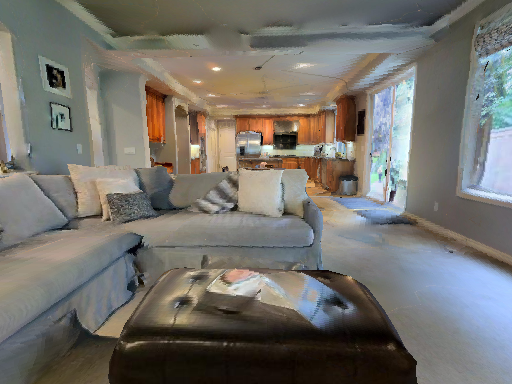
\includegraphics[width=18mm, height=17mm]{TrueDepth/BALLOU/des.png} & 
            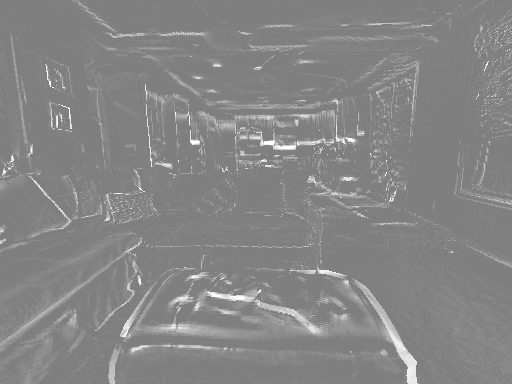
\includegraphics[width=18mm,height=17mm]{PhotoVS/BALLOU/ferror.png} & 
           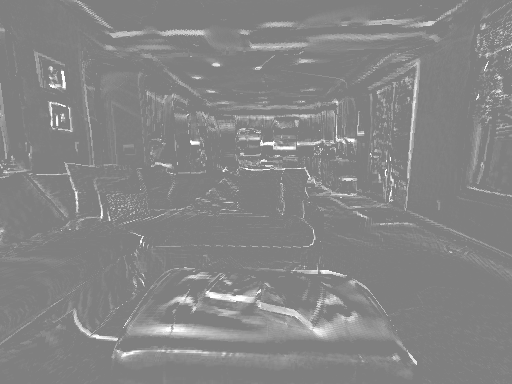
\includegraphics[width=18mm, height=17mm]{ICRA17/BALLOU/ferror.png} & 
 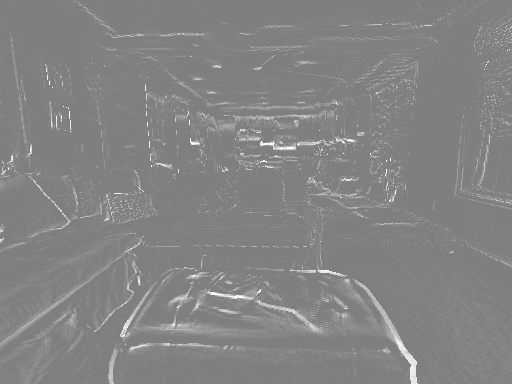
\includegraphics[width=18mm, height=17mm]{TrueDepth/BALLOU/ferror.png} &
  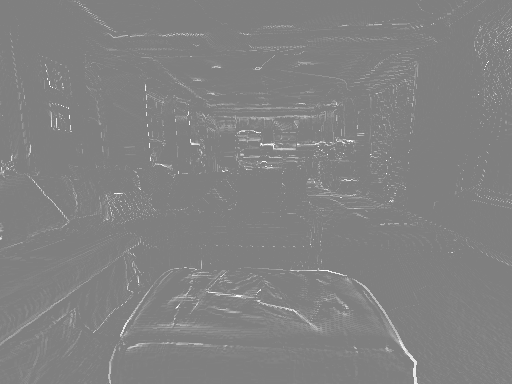
\includegraphics[width=18mm, height=17mm]{DepthNetwork/BALLOU/ferror.png} &
    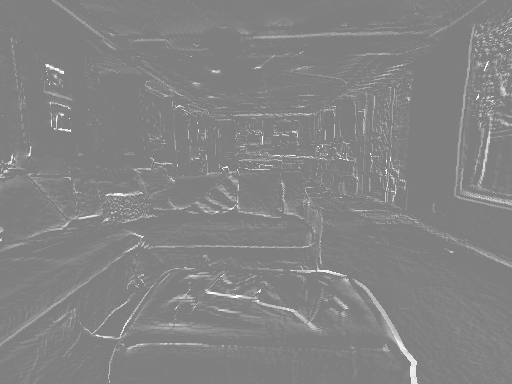
\includegraphics[width=18mm, height=17mm]{FlowDepth/BALLOU/ferror.png}

 \\ \hline
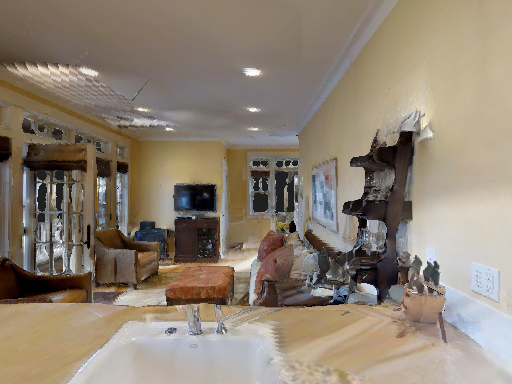
\includegraphics[width=18mm, height=17mm]{TrueDepth/STOKES/init.png} &   
            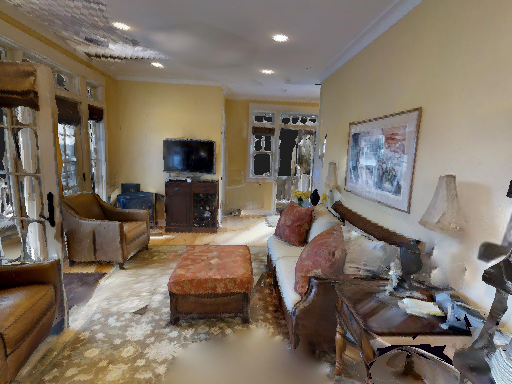
\includegraphics[width=18mm, height=17mm]{TrueDepth/STOKES/des.png} & 
           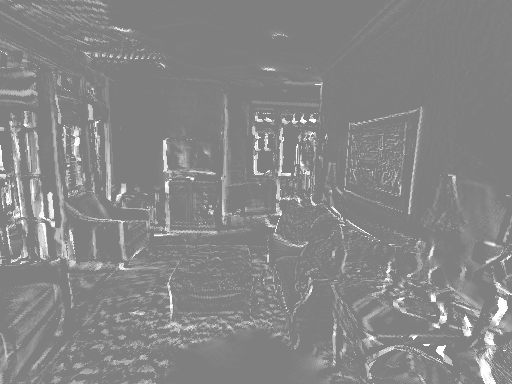
\includegraphics[width=18mm, height=17mm]{PhotoVS/STOKES/ferror.png} & 
           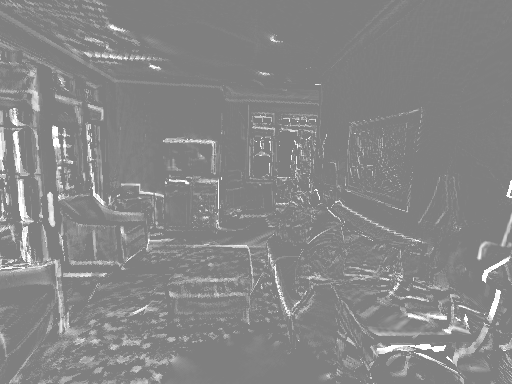
\includegraphics[width=18mm, height=17mm]{ICRA17/STOKES/ferror.png} & 
 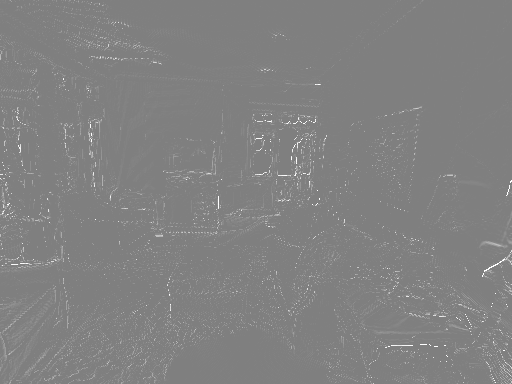
\includegraphics[width=18mm, height=17mm]{TrueDepth/STOKES/ferror.png} &
 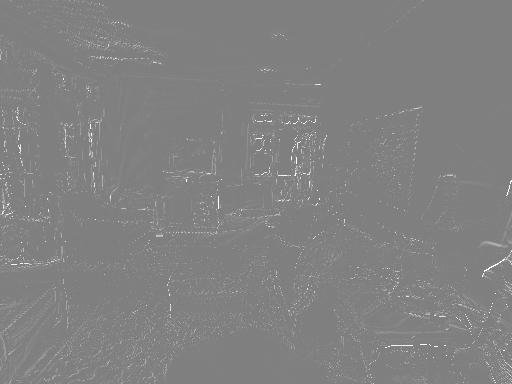
\includegraphics[width=18mm, height=17mm]{DepthNetwork/STOKES/ferror.png}  &
 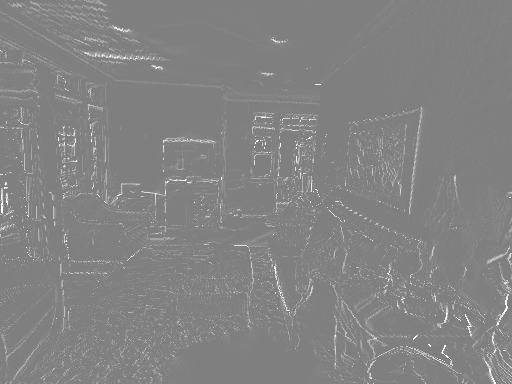
\includegraphics[width=18mm, height=17mm]{FlowDepth/STOKES/ferror.png}  \\ \hline

\hline \hline

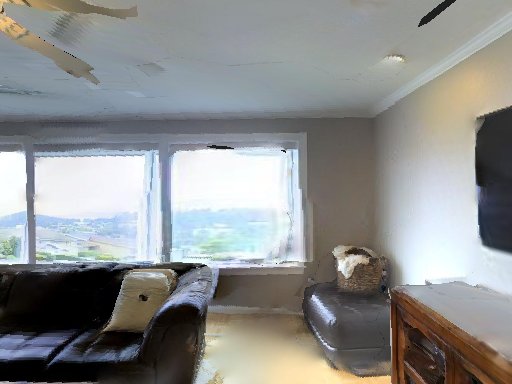
\includegraphics[width=18mm, height=17mm]{TrueDepth/MESIC/init.png} &   
            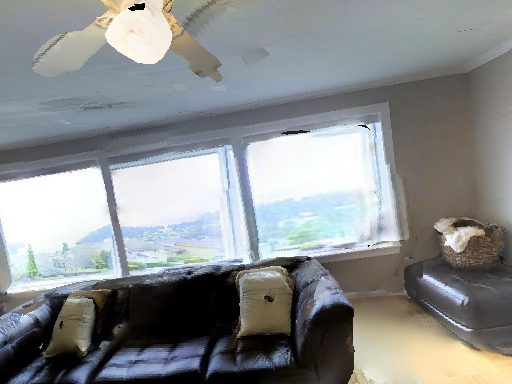
\includegraphics[width=18mm, height=17mm]{TrueDepth/MESIC/des.png} & 
              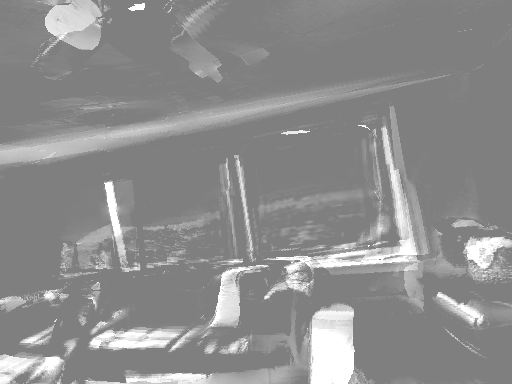
\includegraphics[width=18mm, height=17mm]{PhotoVS/MESIC/ferror.png} &   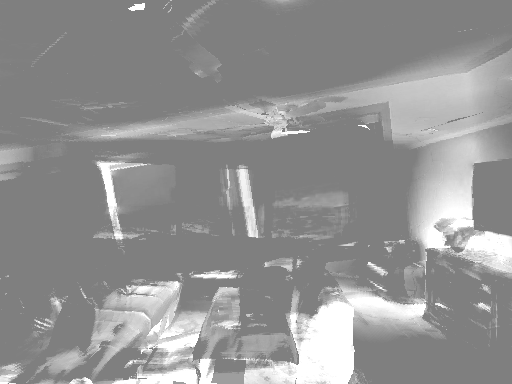
\includegraphics[width=18mm, height=17mm]{ICRA17/MESIC/ferror.png} & 
 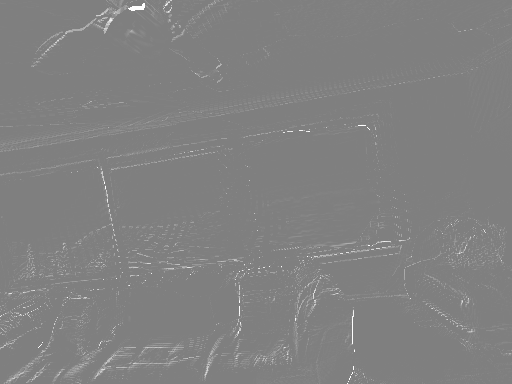
\includegraphics[width=18mm, height=17mm]{TrueDepth/MESIC/ferror.png} &
  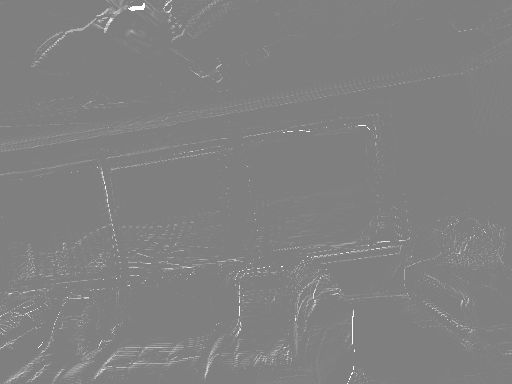
\includegraphics[width=18mm, height=17mm]{DepthNetwork/MESIC/ferror.png} &
   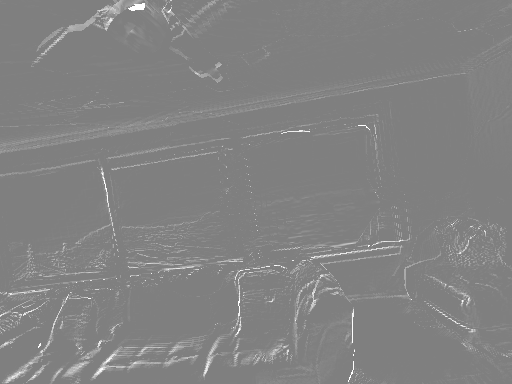
\includegraphics[width=18mm, height=17mm]{FlowDepth/MESIC/ferror.png}
 \\ \hline

  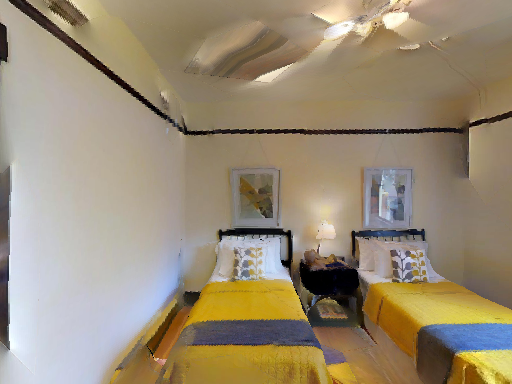
\includegraphics[width=18mm, height=17mm]{TrueDepth/ARKANSAW/init.png} &   
            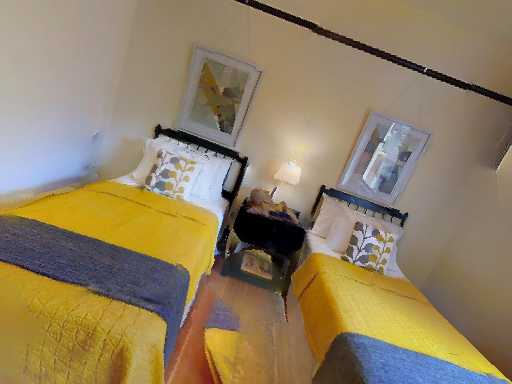
\includegraphics[width=18mm, height=17mm]{TrueDepth/ARKANSAW/des.png} & 
           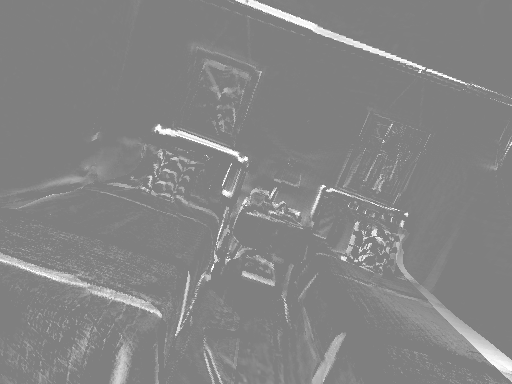
\includegraphics[width=18mm, height=17mm]{PhotoVS/ARKANSAW/ferror.png} & 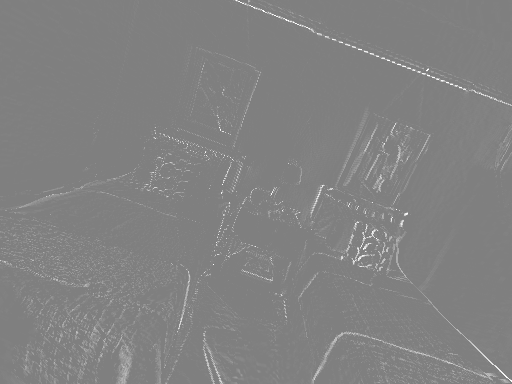
\includegraphics[width=18mm, height=17mm]{ICRA17/ARKANSAW/ferror.png} & 

 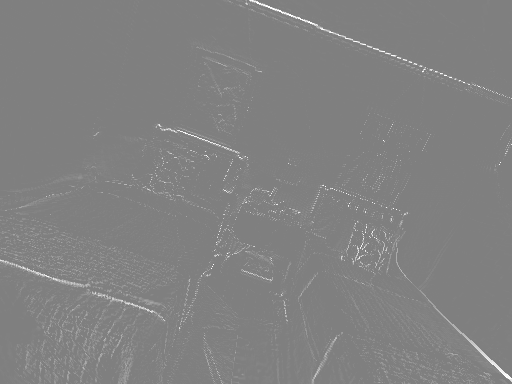
\includegraphics[width=18mm, height=17mm]{TrueDepth/ARKANSAW/ferror.png} &
  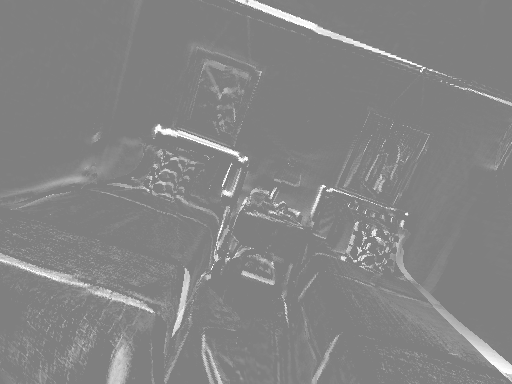
\includegraphics[width=18mm, height=17mm]{DepthNetwork/ARKANSAW/ferror.png} &
    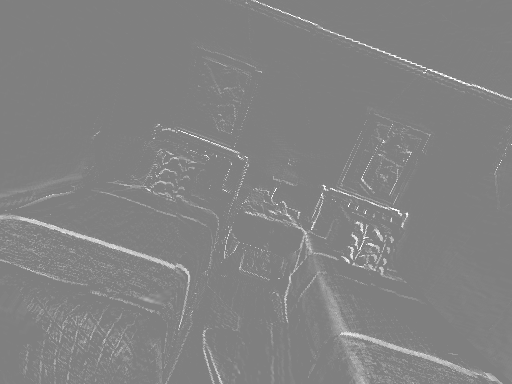
\includegraphics[width=18mm, height=17mm]{FlowDepth/ARKANSAW/ferror.png}
 \\ \hline
 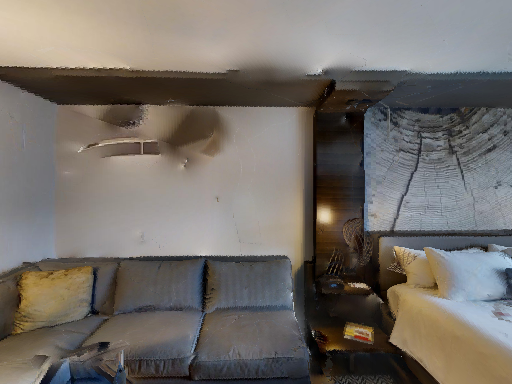
\includegraphics[width=18mm, height=17mm]{TrueDepth/PABLO/init.png} &   
            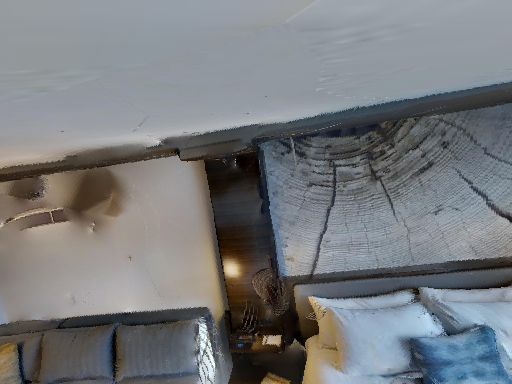
\includegraphics[width=18mm, height=17mm]{TrueDepth/PABLO/des.png} & 
           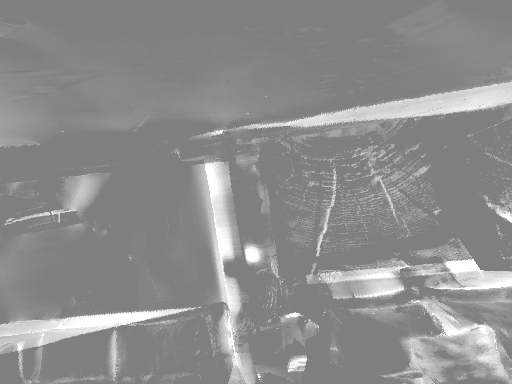
\includegraphics[width=18mm, height=17mm]{PhotoVS/PABLO/ferror.png} & 
           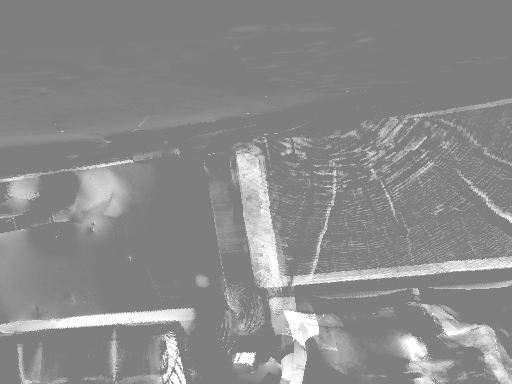
\includegraphics[width=18mm, height=17mm]{ICRA17/PABLO/ferror.png} & 
 \includegraphics[width=18mm, height=17mm]{TrueDepth/PABLO/ferror.png} &
 \includegraphics[width=18mm, height=17mm]{DepthNetwork/PABLO/ferror.png} &
 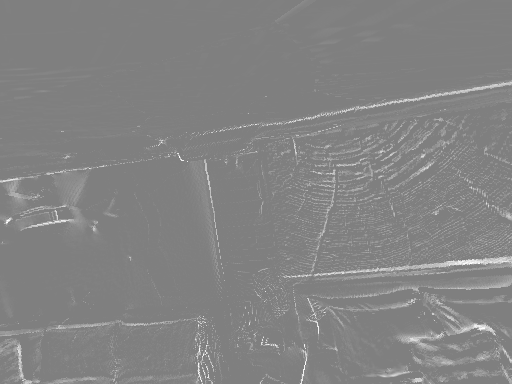
\includegraphics[width=18mm, height=17mm]{FlowDepth/PABLO/ferror.png} 
 \\ \hline
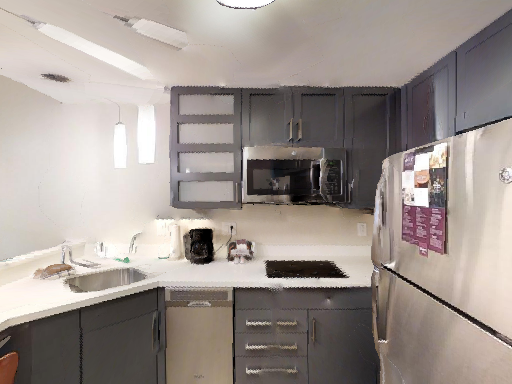
\includegraphics[width=18mm, height=17mm]{TrueDepth/EUDORA/init.png} &   
            \includegraphics[width=18mm, height=17mm]{TrueDepth/EUDORA/des.png} &
           \includegraphics[width=18mm, height=17mm]{PhotoVS/EUDORA/ferror.png} & 

           \includegraphics[width=18mm, height=17mm]{ICRA17/EUDORA/ferror.png} & 
 \includegraphics[width=18mm, height=17mm]{TrueDepth/EUDORA/ferror.png} &
  \includegraphics[width=18mm, height=17mm]{DepthNetwork/EUDORA/ferror.png} &
   \includegraphics[width=18mm, height=17mm]{FlowDepth/EUDORA/ferror.png}
 \\ \hline
\hline \hline
\includegraphics[width=18mm, height=17mm]{TrueDepth/QUANTICO/init.png} &   
            \includegraphics[width=18mm, height=17mm]{TrueDepth/QUANTICO/des.png} & 
           \includegraphics[width=18mm, height=17mm]{PhotoVS/QUANTICO/ferror.png} &\includegraphics[width=18mm, height=17mm]{ICRA17/QUANTICO/ferror.png} & 
 \includegraphics[width=18mm, height=17mm]{TrueDepth/QUANTICO/ferror.png} &
  \includegraphics[width=18mm, height=17mm]{DepthNetwork/QUANTICO/ferror.png} &
    \includegraphics[width=18mm, height=17mm]{FlowDepth/QUANTICO/ferror.png}

 \\ \hline
\includegraphics[width=18mm, height=17mm]{TrueDepth/HILLSDALE/init.png} &   
            \includegraphics[width=18mm, height=17mm]{TrueDepth/HILLSDALE/des.png} & 
           \includegraphics[width=18mm, height=17mm]{PhotoVS/HILLSDALE/ferror.png} & 
           \includegraphics[width=18mm, height=17mm]{ICRA17/HILLSDALE/ferror.png} & 
 \includegraphics[width=18mm, height=17mm]{TrueDepth/HILLSDALE/ferror.png} & 
  \includegraphics[width=18mm, height=17mm]{DepthNetwork/HILLSDALE/ferror.png} &
    \includegraphics[width=18mm, height=17mm]{FlowDepth/HILLSDALE/ferror.png} 

 \\ \hline
\includegraphics[width=18mm, height=17mm]{TrueDepth/DENMARK/init.png} &   
            \includegraphics[width=18mm, height=17mm]{TrueDepth/DENMARK/des.png} &  \includegraphics[width=18mm, height=17mm]{PhotoVS/DENMARK/ferror.png} & 

           \includegraphics[width=18mm, height=17mm]{ICRA17/DENMARK/ferror.png} & 
 \includegraphics[width=18mm, height=17mm]{TrueDepth/DENMARK/ferror.png} &
  \includegraphics[width=18mm, height=17mm]{DepthNetwork/DENMARK/ferror.png} &
   \includegraphics[width=18mm, height=17mm]{FlowDepth/DENMARK/ferror.png}
 \\ \hline
      \end{tabular}
%      \end{adjustbox}
\caption{Qualitative results on the benchmark for 10 scenes. Given initial and desired images of various scenes from the benchmark, we compare 3 variants of our approach (true depth, network-depth and flow-depth) with  Saxena et al. \cite{servonet} and show the error image between desired and resulting pose of the approach. While \cite{servonet} converges on easy scenarios (row 1-3) and sometimes on medium scenarios (row 4-7) and not at converge on hard scenes. All the variants are able to converge on all test-cases.}
 \label{fig:bench_qual}
 \end{center}
 \end{figure*}




\subsection{Controller performance}
For analysing the controller performance, we next present the results for a visual servoing trial. The inail pose and desired pose are given by figure {??} and figure {??}. From figure [??] it can be seen that .....

\begin{figure}
\centering
\begin{tabular}{cc}

\includegraphics[width=4cm, height=3cm]{Plots/Photo_all.eps} &
\includegraphics[width=4cm, height=3cm]{Plots/tvel_all.eps} \\
(a) & (b) \\
\includegraphics[width=4cm, height=3cm]{Plots/rvel_all.eps} &
\includegraphics[width=4cm, height=3cm]{Plots/traj_all.eps}\\
(c) & (d)
\end{tabular}
\caption[3D positioning task]{3D positioning task:
(a)  Translational velocity in m/s.,
(b) Rotational velocity in rad/s.,
(c) Photometric feature error, and
(d) Camera trajectory. Our
approach is able to attain the desired pose even when the displacement
between initial and desired pose is large and lightning is non-homogeneous. }
\label{fig:ex3}%
\end{figure}

\subsection{Convergence study}
Classic visual servoing approaches especially dense visual servoing can attain the goal with sub-milliliter accuracy. However, their convergence basin is limited. One of the major advantages that neural visual servoing   approaches exhibit is in terms of their convergence domain. In this experiment we compare our approach with existing approaches for studying the convergence domain. We select a scene in habitat environment and evaluate how many times our approach was able to converge. To have a fair comparison we follow a similar methodology as suggested by \cite{trainingdeepvs}. It can be seen from the figure\ref{fig:convergence} that our approaches outperforms the existing approaches even in the converge criterion. To complete the study of how good the convergence we further report the convergence domain in terms of camera pose as well as overlap for three scenes for the benchmark.
The above shown pipelines in the graphs were evaluated over 10 batches , each batch with 20 individual runs over 10 different environments in the data set with each environment having fixed initial position. The final position was varied incrementally from batch 0 to 9 by linearly increasing the translation and rotation in  each batch by 0.3 meters and 8 degrees in x, y and z.  
\begin{figure}%
\centering
\includegraphics[width=4cm, height=3cm] {stability_convergence/convergence_2.eps}
\caption{Convergence study for medium and large camera transforms.}
\label{fig:convergence}
\end{figure}
%\subsection{Ablation study}
\subsection{Real drone experiment}
We finally validate the generalisation of our approach on real data using a aerial robot on two different scenarios one outdoor and one indoor. We again test our approach for a large camera transformation as the initial and desired images are given by figure \ref{??} respectively. It can be seen qualitatively that the robot is able to attain the desired pose precisely even though large camera transformation and different illumination conditions for even outdoor scenario without any requirement for fine-tuning or retraining.

\begin{figure}%
\centering
\begin{tabular}{cc}
\includegraphics[width=4cm,height=2cm]{drone/intitial.png} &
\includegraphics[width=4cm,height=2cm]{drone/desired_image.png} \\
(a) & (b) \\
\includegraphics[width=4cm, height=2.5cm]{drone/attained_image.png} &
\includegraphics[width=4cm, height=2.5cm]{drone/drone_initial.png} \\
(c) & (d) \\
\includegraphics[width=4cm, height=2.5cm]{drone/drone_final.png} &
\includegraphics[width=4cm, height=2.5cm]{drone/Drone_traj_small2.pdf} \\
(e) & (f)
\end{tabular}
\caption{Outdoor positioning task: (a) Initial image as seen by the drone, (b) Desired final image (c) Attained image,
(d) Initial drone position as seen by us,
(e) Final drone position as seen by us. and (f) Drone's Trajectory.}

\label{fig:ex3}%
\end{figure}




\section{Conclusion}
In this work, we have put forward a baseline comparison between all the present state of the art visual servoing techniques and have quantified the effect of each method. We have compared our image based visual servoing technique with the existing frameworks for visual servoing tasks using CNN. We have used a network to estimate the optical flow between the images and have used this as visual features in order to estimate the camera velocity and perform servoing accordingly. A major break through in the attainment of the desired pose can be found using the integration of the flow features with a depth network which performs on par with the state of the art depth networks. This method is reliable on a large variety of scenes as the depth network is trained both on indoor and outdoor scenes, therefore our pipeline with IBVS can be deployed in any environmental setting.

\bibliographystyle{IEEEtran}
\bibliography{IEEE}
\end{document}

\section{TODO}
\begin{enumerate}
    \item stability experiments results 
    \item merge figure 4 and 5
    \item if possible add 1 experiment on samll object 
    \item caption all figures
    \item make gitlab/rrc page  
\end{enumerate}




%  \begin{table}[h!]
% \begin{adjustbox}{width=0.5\textwidth,center}   \begin{tabular}{|c|c|c|c|c|c|c|}
% \hline
% Metric & Initial error & Photo VS & Saxena et al. \cite{servonet} & True depth & Depth-net& Flow-depth \\ \hline
% \hline \hline
% Tra. err(m) &1.42 & 0.06 & 0.19 & 0.02 & 0.02 & 0.04 \\\hline
% Rot. err(\deg) & $18.20$ & $0.76$ & $0.89$ & $0.37$ & $0.38$ & $0.72$ \\  \hline
%  Traj len(m) & - &2.26 & 2.69 &  2.24  &  1.42  &  1.19  \\ \hline
%  Iter& - & 956 & 1486   &  764  &  233  &  1560  \\ \hline
% \hline
% Tra. err(m) & 1.79 & 0.12 & 0.08 & 0.04 & 0.02 & 0.03 \\\hline
% Rot. err(\deg) & 16.33 & 0.66 & 0.84 & 0.84 & 0.42 & 0.06 \\  \hline
%  Traj len(m) & - & 2.22 & 2.48  &  1.58  &  1.55  &  2.31  \\ \hline
%  Iter& - & 869 &  1687  &  150  &  143  &  871  \\ \hline
% \hline
% Tra. err(m) &1.64 & 0.33 & 0.04 & 0.03 & 0.03 & 0.03 \\ \hline
% Rot. err(\deg)& 30.96 & 3.57 & 1.39 & 0.85 & 0.83 & 0.89 \\  \hline
%  Traj len(m) & - & NC & 2.86  &  2.36  &  3.65  &  2.37 \\ \hline
%  Iter&- & NC & 1235  &  84  &  89  &  869  \\ \hline
% \hline

% \hline  \hline
% Tra. err(m) &1.95 & 0.54 & 0.35 & 0.02 & 0.02 & 0.03 \\ \hline
% Rot. err(\deg)& 22.86 & 4.56 & 6.47 & 0.53 & 0.53 & 1.39 \\  \hline
%  Traj len(m) &- & NC & NC  &  2.74  &  2.82  &  1.85  \\ \hline
%  Iter& - & - & -  &  62  &  244  &  981  \\ \hline
% \hline
% Tra. err(m) &1.41 & 0.28 & 0.13 & 0.04 & 0.02 & 0.04 \\\hline
% Rot. err(\deg)& 18.07 & 3.23 & 6.44 & 8.72 & 8.87 & 8.39 \\  \hline
%  Traj len(m) &  - & NC & 2.94  &  2.31  &  1.19  &  1.1 \\ \hline
%  Iter& - & - & 1647  &  214  &  185  &  580  \\ \hline
% \hline
% Tra. err(m) &1.15 & 0.91 & 0.83 & 0.02 & 0.02 & 0.02 \\ \hline
% Rot. err(\deg)& 17.27 & 13.25 & 10.54 & 1.39 & 1.38 & 0.66 \\  \hline
%  Traj len(m) & - & NC & NC  &  1.52  &  2.56  &  0.89  \\ \hline
%  Iter& - & - &-  &  104  &  186  &  3831  \\ \hline
% \hline
% Tra. err(m) &1.37 & 1.29 & 1.25 & 0.03 & 0.02 & 0.01 \\\hline
% Rot. err(\deg)& 17.26 & 7.63 & 9.55 & 1.81 & 0.77 & 1.81 \\  \hline
%  Traj len(m) & - & NC & NC  &  1.33  &  2.49  &  1.26  \\ \hline
%  Iter& - & - & -  &  20  &  283  &  661  \\ \hline

% \hline \hline
% Tra. err(m) &2.54 & 2.49 & 2.32 & 0.03 & 0.01 & 0.02 \\\hline
% Rot. err(\deg)& 20.02 & 39.65 & 48.77 & 11.67 & 0.34 & 0.55 \\  \hline
%  Traj len(m) & - & NC & NC  &  2.03  &  5.88  &  2.26  \\ \hline
%  Iter& - & - & 0  &  504  &  237  &  754  \\ \hline
% \hline
% Tra. err(m) &1.94 & 2.36 & 2.27 & 0.04 & 0.041 & 0.041 \\ \hline
% Rot. err(\deg)& 31.78 & 43.37 & 29.69 & 0.78 & 0.75 & 0.91 \\  \hline
%  Traj len(m) &  - & NC & NC  &  2.24  &  2.28  &  2.32  \\ \hline
%  Iter& - & -& -  &  183  &  145  & 1124  \\ \hline
% \hline
% Tra. err(m) &2.43 & 2.27 & 1.36 & 0.01 & 0.0 & 0.02 \\ \hline
% Rot. err(\deg)& 36.05 & 53.246 & 29.24 & 0.28 & 0.16 & 0.49 \\  \hline
%  Traj len(m) & - & NC &NC  &  $2.52$  &  2.67  &  3.52  \\ \hline
%  Iter& - & -& -  &  314  &  114  &  1386  \\ \hline

%       \end{tabular} 
%              \end{adjustbox}
% \caption{Comparitive Table of Rotational and Translational errors in poses}
%  \label{tbl:bench_quant}
%  \end{table}


